\documentclass[10pt]{manual}

% Input encoding and typographical rules for English language
\usepackage[utf8]{inputenc}
\usepackage[english]{babel}
\usepackage[english]{isodate}

\usepackage{array}
\usepackage{bigdelim}

\newcolumntype{C}[1]{>{\centering\arraybackslash}p{#1}}

\usepackage{tikz}
\usepackage{pgfplots}
\usepackage{circuitikz}
\usetikzlibrary{calc}
\pgfplotsset{compat=1.16}
\pgfkeys{/pgf/number format/.cd,1000 sep={\,}}

% These define global texts that are used in headers and titles.
\title{DEDP-100 Differential Probe}
\subtitle{User Manual}
\author{devEmbedded}
\date{June 2021}
\revision{Preliminary}
\companylogo{\includegraphics[width=60mm]{devembedded.pdf}}

\begin{document}
\maketitle
\newpage

\section{Introduction}

A differential probe measures the voltage difference between the two input contacts.
Unlike a regular oscilloscope probe, neither of the contacts have a direct connection to ground.
This allows measurements of circuits that have a different reference potential than the oscilloscope ground is.

\section{Parts and functionality}

The DEDP-100 Differential Probe consists of a differential amplifier,
detachable input accessories and a triaxial cable to oscilloscope.
The triaxial cable contains an inner 50 ohm coaxial cable to pass the output signal and an outer shield that carries supply current for the amplifier.
The USB power supply connector can be connected to oscilloscope USB port or a separate 5 VDC power supply.

\includegraphics[width=17cm]{perspective_view.pdf}

The amplifier has fixed differential gain settings of 2x and 20x gain and input voltage range of $\pm3\,V$.
The actual measurement range and total system gain is set by a divider included in input accessories.
Two coaxial MCX connectors are provided on the front for attaching shielded cable accessories.
Alternatively, two slots with spring loaded contacts accept tweezer tip accessories.
In both types of accessories, the input divider is located near the probe end, to minimize stray capacitance.

\section{Electrical specifications}

\begin{threeparttable}
\begin{tabularx}{\textwidth}{p{4cm} | C{1.85cm} | C{1.85cm} | C{1.85cm} | X}
\thickhline
&\multicolumn{3}{c|}{\textbf{Accessory divider ratio}}\\
\textbf{Input specification} & \textbf{1:1} & \textbf{1:20} & \textbf{1:200} & \textbf{Conditions}\\
\hline
Resistance & $500\,k\Omega$ & $10\,M\Omega$ & $50\,M\Omega$ & \rdelim\}{2.9}{*}\multirow{3}{*}{Each input relative to output GND} \\
Capacitance & 10-30 pF & 2 pF & 2 pF &  \\
Total voltage & $\pm3.0\,V$ & $\pm60\,V$ & $\pm600\,V$ & \\
Differential voltage & $\pm1.8\,V$ & $\pm36\,V$ & $\pm360\,V$ & 2x differential gain selection\\
                     & $\pm0.18\,V$ & $\pm3.6\,V$ & $\pm36\,V$ & 20x differential gain selection\\
Oscilloscope probe setting & 0.5x & 10x & 100x & 2x gain \\
                           & 0.05x & 1x & 10x & 20x gain \\
\thickhline
\end{tabularx}
\end{threeparttable}

\begin{threeparttable}
\begin{tabularx}{\textwidth}{p{4cm} | C{3cm} | C{3cm} | X}
\thickhline
&\multicolumn{2}{c|}{\textbf{Differential gain setting}} \\
\textbf{AC specification} & \textbf{2x} & \textbf{20x} & \textbf{Conditions} \\
\hline
Bandwidth & DC to 20 MHz  & DC to 5 MHz & $\pm0.2\,dB$ gain flatness \tnote{2}\\
          & $\geq50\,MHz$ & $\geq10\,MHz$ & -1 dB gain drop \tnote{1}\\
          & $\geq100\,MHz$ & $\geq20\,MHz$ & -3 dB gain drop \tnote{1}\\
Rise time & 3 ns & 20 ns & 10\% to 90\% \\
Propagation delay & 8 ns & 15 ns & Includes 5 ns cable delay \\
Common mode rejection \tnote{2} & $\geq50\,dB$ & $\geq50\,dB$ & $\leq1\,kHz$ \\
                                & $\geq45\,dB$ & $\geq45\,dB$ & $\leq1\,MHz$ \\
                                & $\geq30\,dB$ & $\geq40\,dB$ & $\leq10\,MHz$ \\
                                & $\geq20\,dB$ & $\geq30\,dB$ & $\leq100\,MHz$ \\
\thickhline
\end{tabularx}
\end{threeparttable}

\begin{threeparttable}
\begin{tabularx}{\textwidth}{p{4cm} | C{3cm} | C{3cm} | X}
\thickhline
&\multicolumn{2}{c|}{\textbf{Differential gain setting}} \\
\textbf{Output specification} & \textbf{2x} & \textbf{20x} & \textbf{Conditions} \\
\hline
Gain accuracy & $\pm2\%$ & $\pm2\%$ & \\
Noise & $5\,mV_{p-p}$ & $15\,mV_{p-p}$ & \\
Offset \tnote{2} & $\pm1\,mV$ & $\pm1\,mV$ & 10 minutes warm-up \\
Offset drift & $\pm5\,mV$ & $\pm5\,mV$ & $10\degree C$ to $40\degree C$\\
Maximum voltage & $\pm6.0\,V$ & $\pm6.0\,V$ & \\
\thickhline
\end{tabularx}
\end{threeparttable}

\begin{threeparttable}
\begin{tabularx}{\textwidth}{p{4cm} | C{6.45cm} | X}
\thickhline
\textbf{Supply specification} & \textbf{Value} & \textbf{Conditions}\\
\hline
Supply voltage & 3.5 -- 5.5 V \\
Operating current & 300 mA & 5.0 V, typical\\
                  & 500 mA & 3.5 V, maximum\\
\thickhline
\end{tabularx}
\begin{tablenotes}
    \item[1] {Output swing 300 mVp-p to $50\,\Omega$ termination, see figure \ref{fig_termination}.}
    \item[2] {After adjustment described on page \pageref{adjustment}.}
\end{tablenotes}
\end{threeparttable} 

\section{Adjustment after accessory change}
\label{adjustment}
This differential probe can be adapted to different measurement ranges by using interchangeable probe accessories.
Because of component tolerances, an adjustment procedure is required after accessory change to achieve the best
frequency response flatness, common mode rejection and output offset performance.

Adjustment is performed by two trimmer capacitors and two trimmer resistors, accessible through holes in the top cover.
The trimmer capacitors are marked \textbf{AC+} and \textbf{AC-} and adjust the high-frequency gain to make it equal to low-frequency gain.
The trimmer resistors are marked \textbf{DC balance} and \textbf{DC offset} and adjust the low frequency characteristics.
Suitable adjustment tool is 1.5 mm wide flat head screwdriver.
Both conductive and non-conductive tools are suitable.

Adjustment requires use of a square wave source.
Most oscilloscopes include a calibration output that is suitable for the purpose.
A signal generator can also be used: set it to square wave, 1 kHz, 3 Vp-p.
If a separate signal generator is used, connect its ground terminal to oscilloscope ground.

\begin{enumerate}
\item \textbf{Frequency response flatness:} Connect positive input probe to square wave signal and negative to ground.
\begin{enumerate}
\item Set probe gain switch to 2x.
\item Set oscilloscope vertical scale and timebase so that the signal is visible.
\item Adjust \textbf{AC+} until rising signal edges are sharp without overshoot (see figure X).
\end{enumerate}
\item \textbf{Common mode rejection:} Connect both positive and negative probe to square wave signal.
\begin{enumerate}
\item Set probe gain switch to 20x.
\item Set oscilloscope vertical scale to 100 mV/div.
\item Adjust \textbf{AC-} until rising edge spikes of the signal are removed.
\item Adjust \textbf{DC balance} until the displayed signal is a flat line (see figure X).
\end{enumerate}
\item \textbf{DC offset:}
\begin{enumerate}
\item Set probe gain switch to the setting you will use for measurements.\\There is a small difference in offset between the gain settings.
\item Adjust \textbf{DC offset} until output signal is 0 V.
\end{enumerate}
\end{enumerate}

\section{Oscilloscope settings}
\subsection{Termination impedance}
The differential amplifier has $50\,\Omega$ output impedance.
It is compatible with both $1\,M\Omega$ or $50\,\Omega$ impedance oscilloscope inputs.
Using $50\,\Omega$ termination is recommended for measurement of signals with frequency higher than 20 MHz,
as it removes gain fluctuations caused by reflections in the signal cable.
Using $1\,M\Omega$ termination is recommended for signals with amplitude below 1\% of total range,
as it doubles the signal level visible at the oscilloscope input.
Figure \ref{fig_termination} shows the frequency response with both termination types.

Many high bandwidth oscilloscopes have a software option to select the termination impedance.
For oscilloscopes without this setting, an inline $50\,\Omega$ terminator such as P57 or Cal Test CT2944 can be used.

\begin{figure}[h]
    \sffamily
    \begin{tikzpicture}
        \begin{axis}[
            width=15cm,
            height=6cm,
            xlabel={Frequency (MHz)},
            ylabel={Relative gain (dB)},
            ytick distance=1,
            xtick distance=50,
            ymin=-3, ymax=1,
            xmin=0, xmax=180,
            minor y tick num = 4,
            minor x tick num = 4,
            xmajorgrids, ymajorgrids, xminorgrids, yminorgrids,
            major grid style = {darkgray, thin},
            minor grid style = {lightgray, very thin},
            enlarge x limits = 0,
            legend style = {draw = none, legend pos = north east}
        ]
        \addplot [mark=none, draw=black, thick] table
            [col sep = semicolon, x expr = {(\thisrowno{0}) * 1e-6}, y expr = {20*log10(\thisrowno{1}) - 0.5}]
            {response_1Mohm.txt};
        \addlegendentry{$1\,M\Omega$ termination};
        \addplot [mark=none, draw=blue, very thick] table
            [col sep = semicolon, x expr = {(\thisrowno{0}) * 1e-6}, y expr = {20*log10(\thisrowno{1}) + 5.6}]
            {response_50ohm.txt};
        \addlegendentry{$50\,\Omega$ termination};
        \end{axis}
    \end{tikzpicture}
    \caption{Frequency response dependence on oscilloscope termination impedance.}
    \label{fig_termination}
\end{figure}

\subsection{Probe ratio}
Most digital oscilloscopes contain a probe ratio setting to display correct voltages for on-screen measurements.
For this differential probe, the total attenuation ratio and thus the correct oscilloscope setting depend on three parameters:

\begin{enumerate}
\item Input accessory attenuation ratio, typically 1:20 or 1:200.
\item Differential gain switch setting, either 2x or 20x.
\item Oscilloscope termination attenuation, which is 1:1 for $1\,M\Omega$ termination and 1:2 for $50\,\Omega$ termination.
\end{enumerate}

The table below shows the correct oscilloscope setting for most common configurations:

\begin{tabularx}{\textwidth}{l|C{2cm}|C{2cm}|X}
\thickhline
& \multicolumn{2}{c|}{\textbf{Accessory ratio}} \\
& \textbf{1:20} & \textbf{1:200} \\
\hline
\textbf{2x gain} & 10x & 100x & \rdelim\}{1.9}{*}\multirow{2}{*}{$1\,M\Omega$ termination} \\
\textbf{20x gain} & 1x & 10x &  \\
\hline
\textbf{2x gain} & 20x & 200x & \rdelim\}{1.9}{*}\multirow{2}{*}{$50\,\Omega$ termination} \\
\textbf{20x gain} & 2x & 20x &  \\
\thickhline
\end{tabularx}

\section{Accessories}
\subsection{1:20 tweezer tips}

\begin{tabularx}{\textwidth}{cX}
    \raisebox{-4mm}{\warning} & The tweezer tip accessory is suitable only for measurement of safe low voltage circuits. Do not use it with circuits connected to hazardous voltages. \\
\end{tabularx}

The tweezer tip accessory is designed for measurement of low voltage signals on printed circuit boards.
The tips have a gold plated contact surface on the inside and an insulating surface on the outside.
This allows inserting the tip between integrated circuit leads without causing a short-circuit.
For hands-free usage, a rubber band or a piece of heatshrink tubing can be used to keep the tweezer closed around a component.

The divider circuit is placed close to the tip to minimize parasitic capacitance.
It consists of a $110\,\Omega$ series damping resistor, $9.53\,M\Omega$ divider resistor and $2.0\,pF$ compensation capacitor.

To install the detachable tweezer tips, push them firmly into slots on the sides of the amplifier enclosure.
Verify that the tweezer ends meet when pressed together.
To remove, pull straight outwards to release the taper fit.
Remove tweezer tips when using a cable accessory, as having two accessories simultaneously connected will affect the frequency response.

The gold coating on the tips may wear out in heavy use.
The tips can be resharpened using a file or sand paper to remove the worn out part.

\begin{itemize}
\item \textbf{Measurement range (common mode + differential)}: $\pm60\,V$ to output GND
\item \textbf{Measurement range (differential): $\pm36\,V$}
\item \textbf{Absolute maximum voltage}: $\pm150\,V$ to output GND
\item \textbf{Measurement category}: 60 V -- CAT I (circuits not connected to mains)
\item \textbf{Input capacitance (nominal)}: 1.5 pF each side to GND
\item \textbf{Input capacitance (in typical measurement setup)}: 3 pF each side to GND, 3 pF differential
\item \textbf{Input resistance}: $10\,M\Omega$ each side to GND
\end{itemize}

\begin{figure}[h]
    \sffamily
    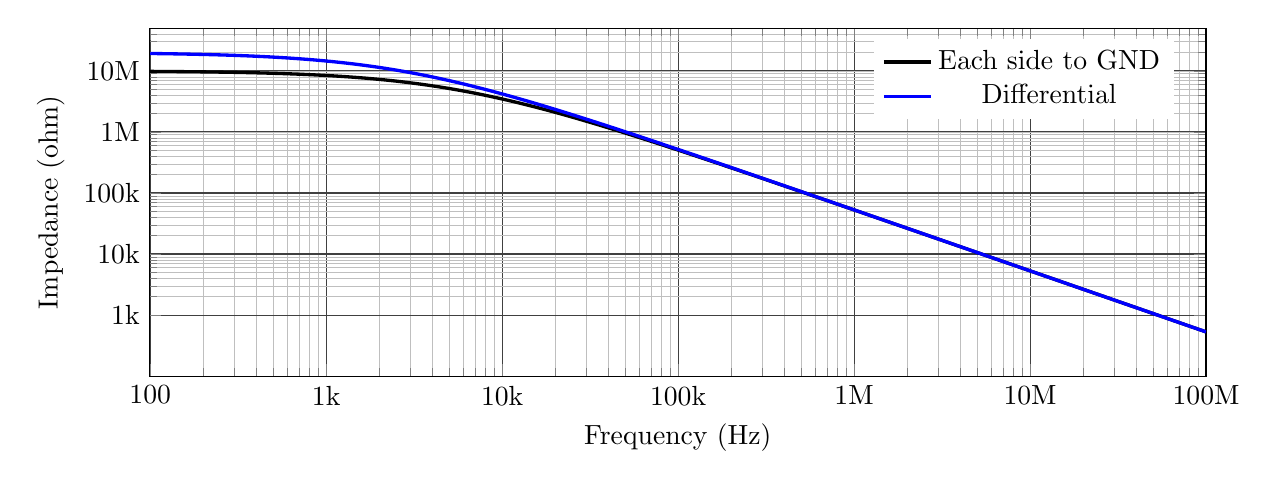
\begin{tikzpicture}
        \begin{loglogaxis}[
            width=15cm,
            height=6cm,
            xlabel={Frequency (Hz)},
            ylabel={Impedance (ohm)},
            ytick distance=10,
            xtick distance=10,
            ymin=100, ymax=50e6,
            xmin=99, xmax=100e6,
            xtick={1e2,1e3,1e4,1e5,1e6,1e7,1e8},
            xticklabels={100,1k,10k,100k,1M,10M,100M},
            ytick={1e3,1e4,1e5,1e6,1e7,1e8},
            yticklabels={1k,10k,100k,1M,10M,100M},
            xmajorgrids, ymajorgrids, xminorgrids, yminorgrids,
            major grid style = {darkgray, thin},
            minor grid style = {lightgray, very thin},
            enlarge x limits = 0,
            legend style = {draw = none, legend pos = north east}
        ]
        % Input impedance consists of the parallel capacitance and resistance.
        \addplot [mark=none, draw=black, very thick, domain=100:100e6, samples=100]
        {
            1 / (2 * pi * x * 3e-12 + 1/10e6)
        };
        \addlegendentry{Each side to GND}
        \addplot [mark=none, draw=blue, very thick, domain=100:100e6, samples=100]
        {
            1 / (2 * pi * x * 3e-12 + 1/20e6)
        };
        \addlegendentry{Differential}
        \end{loglogaxis}
    \end{tikzpicture}
    \caption{Input impedance of 1:20 tweezer tips in typical measurement setup: tweezers held in hand, fingers midway, tips 2 mm apart.}
\end{figure}

\begin{figure}[h]
    \sffamily
    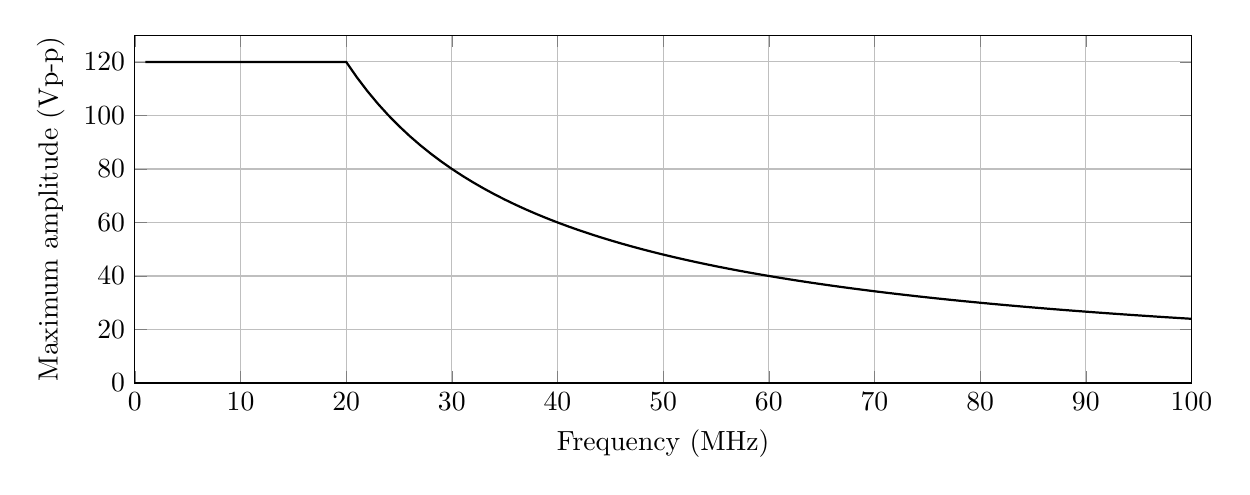
\begin{tikzpicture}
        \begin{axis}[
            width=15cm,
            height=6cm,
            xlabel={Frequency (MHz)},
            ylabel={Maximum amplitude (Vp-p)},
            ytick distance=20,
            xtick distance=10,
            ymin=0, ymax=130,
            xmin=0, xmax=100,
            xmajorgrids, ymajorgrids,
            enlarge x limits = 0
        ]
        % Maximum voltage is limited by power dissipation in the 110 ohm series resistor.
        % The limit for the 0603 resistor is 0.1 W.
        \addplot [mark=none, draw=black, thick, domain=1:100, samples=100]
        { (sqrt(0.1 / 110 * (110 + 1 / (6.28 * 2e-6 * x)^2)) < 120) ?
           sqrt(0.1 / 110 * (110 + 1 / (6.28 * 2e-6 * x)^2)) : 120 };
        \end{axis}
    \end{tikzpicture}
    \caption{Voltage-frequency derating curve for 1:20 tweezer tips}
\end{figure}

\subsection{1:20 cable to square pin socket}

\begin{figure}[h]
    \sffamily
    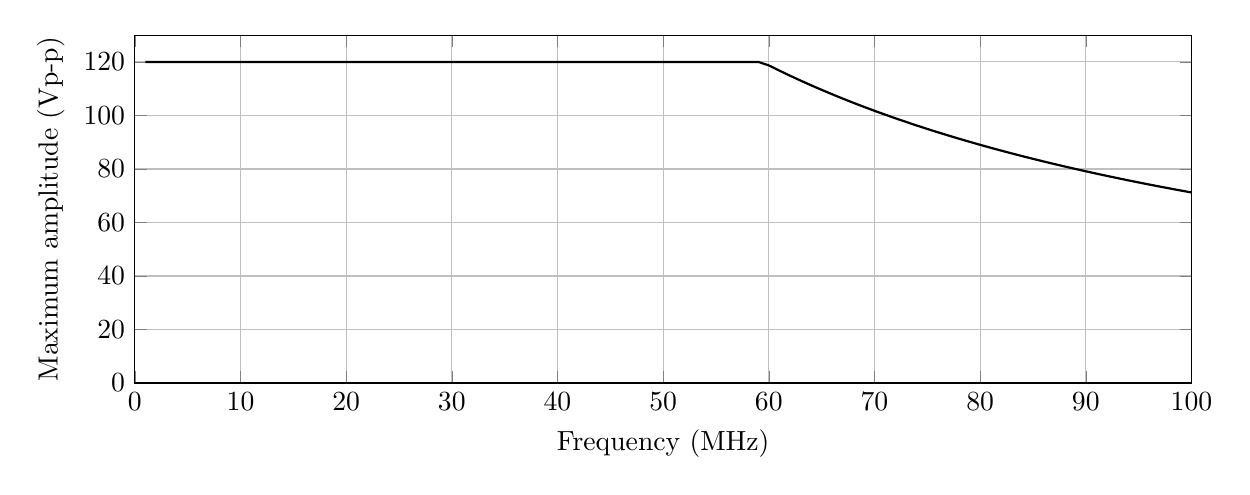
\begin{tikzpicture}
        \begin{axis}[
            width=15cm,
            height=6cm,
            xlabel={Frequency (MHz)},
            ylabel={Maximum amplitude (Vp-p)},
            ytick distance=20,
            xtick distance=10,
            ymin=0, ymax=130,
            xmin=0, xmax=100,
            xmajorgrids, ymajorgrids,
            enlarge x limits = 0
        ]
        % Maximum voltage is limited by power dissipation in the 50 ohm cable attachment series resistor.
        % Due to cable capacitance, only about 50% of current goes through it.
        % The limit for the 0603 resistor is 0.1 W.
        \addplot [mark=none, draw=black, thick, domain=1:100, samples=100]
        { (2 * sqrt(0.1 / 50 * (50 + 1 / (6.28 * 2e-6 * x)^2)) < 120) ?
           2 * sqrt(0.1 / 50 * (50 + 1 / (6.28 * 2e-6 * x)^2)) : 120 };
        \end{axis}
    \end{tikzpicture}
    \caption{Voltage-frequency derating curve for 1:20 cable accessory}
\end{figure}

\subsection{1:200 cable to banana plug}

\begin{itemize}
    \item \textbf{Measurement range (common mode + differential)}: $\pm600\,V$ to output GND
    \item \textbf{Measurement range (differential): $\pm360\,V$}
    \item \textbf{Absolute maximum voltage}: $\pm5000\,V$ to output GND
    \item \textbf{Measurement category}: 600 V -- CAT II (circuits in mains appliances, not for fixed installations)
    \item \textbf{Input capacitance}: 2.0 pF each side to GND
    \item \textbf{Input resistance}: $50\,M\Omega$ each side to GND
\end{itemize}

\begin{figure}[h]
    \sffamily
    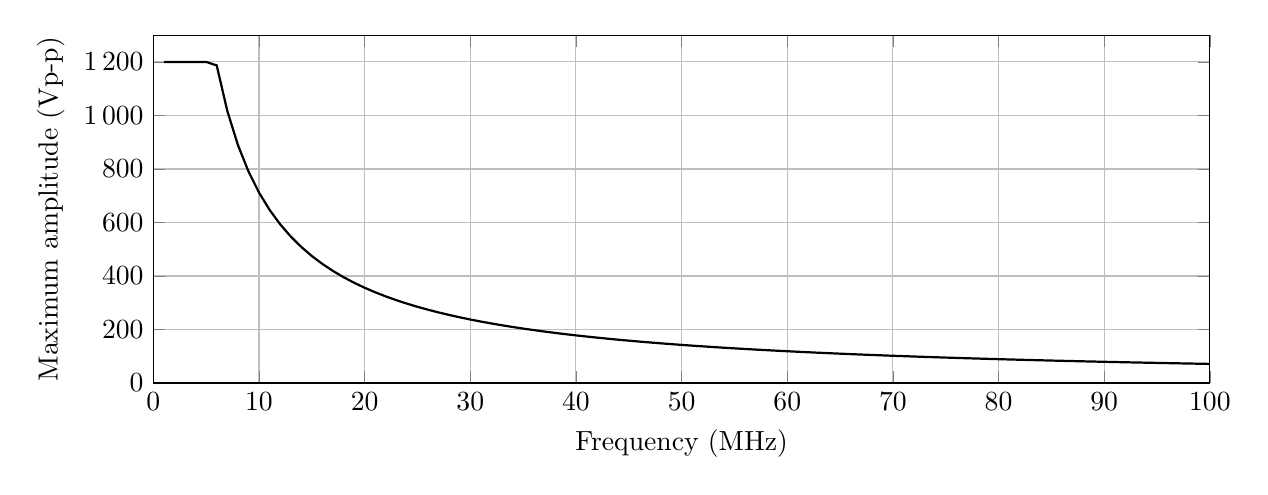
\begin{tikzpicture}
        \begin{axis}[
            width=15cm,
            height=6cm,
            xlabel={Frequency (MHz)},
            ylabel={Maximum amplitude (Vp-p)},
            ytick distance=200,
            xtick distance=10,
            ymin=0, ymax=1300,
            xmin=0, xmax=100,
            xmajorgrids, ymajorgrids,
            enlarge x limits = 0
        ]
        % Maximum voltage is limited by power dissipation in the 50 ohm cable attachment series resistor.
        % It still dominates over the capacitor ESR even though only 5% of current goes through it
        % to the 20 pF amplifier capacitance.
        % The limit for the 0603 resistor is 0.1 W.
        \addplot [mark=none, draw=black, thick, domain=1:100, samples=100]
        { (20*sqrt(0.1 / 50 * (50 + 1 / (6.28 * 20e-6 * x)^2)) < 1200) ?
           20*sqrt(0.1 / 50 * (50 + 1 / (6.28 * 20e-6 * x)^2)) : 1200 };
        \end{axis}
    \end{tikzpicture}
    \caption{Voltage-frequency derating curve for 1:200 cable accessory}
\end{figure}

\begin{tabularx}{\textwidth}{cX}
    \raisebox{-4mm}{\warning} & Ensure that the output BNC connector is connected to a grounded oscilloscope before connecting the input probes. \\
\end{tabularx}

\section{Maintenance and repair}
\section{Mechanical specifications}
\section{Warnings and disclaimers}
This device is intended for use in dry indoor environments.
Only experienced users should perform measurements on circuits that have voltages exceeding $30\,V_{AC}$ or $60\,V_{DC}$, as accidental contact poses a risk of electrocution.
Observe the voltage limits of the accessories used in the measurement setup.

This device is not intended for use in a medical setting or for any safety critical applications.

This device is not suitable as the sole means of determining the absence of hazardous voltage in a circuit.
Always disconnect high voltage supplies before access and if unsure, verify disconnection with another measurement device.

The design of this product is open hardware licensed under CC-BY-4.0 and can be used by other manufacturers with or without customizations.
The specifications in this user manual apply only to original DEDP-100 model manufactured by devEmbedded.

\section{Regulatory compliance}
This product is built in compliance with the following EU standards and directives:

\begin{itemize}
    \item \textbf{EN 61010-1:2010}: Safety requirements for electrical equipment for measurement,\\control, and laboratory use
    \item \textbf{EN 61010-2-030:2010}: Particular requirements for testing and measuring circuits.
    \item \textbf{EN 61326-1:2013}: Electrical equipment for measurement, control and laboratory use \\ - EMC requirements.
    \item \textbf{2011/65/EU}: Restriction of the use of certain Hazardous Substances
    \item \textbf{2014/30/EU}: Electromagnetic Compatibility Directive
\end{itemize}

\end{document}
